\documentclass{article}

\usepackage{neurips_2026}

\usepackage[utf8]{inputenc}
\usepackage[T1]{fontenc}
\usepackage{hyperref}
\usepackage{url}
\usepackage{booktabs}
\usepackage{amsfonts}
\usepackage{amsmath}
\usepackage{amssymb}
\usepackage{nicefrac}
\usepackage{microtype}
\usepackage{xcolor}
\usepackage{graphicx}
\usepackage{subfigure}
\usepackage{tabularx}

\title{Remix, Don't Expand: Chunked Template Routing for Compute-Efficient Transformers}

\author{%
  Anonymous Author(s)\\
  Affiliation\\
  Address\\
  \texttt{email}
}

\begin{document}
\maketitle

\begin{abstract}
Scaling Transformer language models by widening dense linear layers increases both parameter count and inference cost proportionally. Mixture-of-Experts (MoE) architectures decouple these by routing tokens to discrete expert subnetworks, but introduce load-balancing complexity and often underperform dense baselines at small-to-medium scale. We introduce \textbf{RemixedLinear}, a drop-in replacement for standard linear layers that dynamically mixes $K$ learned template matrices per chunk of tokens using lightweight content-aware routing. Each token's effective linear operator is a context-dependent combination of shared templates, gated by a centered output gate ($1 + \tanh$) that preserves dense-equivalent outputs from initialization. Routing is amortized over 64-token chunks and requires no auxiliary load-balancing loss. Through 29 phases of systematic ablation, we identify the key design choices that enable dynamic linear layers to outperform static baselines: chunk-amortized routing, identity-preserving initialization, and applying template mixing at every projection of the block rather than the feed-forward network alone. At depth 12 ($\sim$290M active parameters), RemixedLinear achieves \textbf{0.814 bits-per-byte} compared to 0.903 for the dense baseline at matched active FLOPs, a 10\% improvement. Standard MoE with equivalent routing underperforms the dense baseline. These results hold across three model scales (d4, d8, d12) following a consistent power-law improvement over dense scaling curves.
\end{abstract}

\section{Introduction}

Linear transformations dominate both the parameter count and computational cost of Transformer language models \citep{vaswani2017attention}. As models scale, improving the efficiency of these layers becomes critical for practical deployment. Two broad strategies have emerged: static compression methods such as low-rank factorization \citep{hu2021lora}, which reduce parameters but restrict all inputs to a fixed subspace; and sparse routing methods such as Mixture-of-Experts \citep{shazeer2017outrageously, fedus2022switch}, which activate only a subset of parameters per token but introduce routing instability, load-balancing overhead, and often require substantially larger total parameter counts.

We introduce \textbf{RemixedLinear}, a linear layer that stores $K$ learned template matrices and dynamically composes them per chunk of tokens using content-aware routing. Unlike standard MoE, which routes entire tokens to discrete expert subnetworks at the feed-forward network (FFN) level, RemixedLinear operates at the level of individual linear projections (Q, K, V, projection, and both FFN layers), providing finer-grained dynamic computation. Unlike static low-rank layers, each token induces a distinct full-rank effective operator via continuous template mixing.

The design of RemixedLinear was shaped by 29 phases of systematic ablation. Early designs based on content-dependent multiplicative gating consistently failed due to what we term \emph{optimization friction}: the gradient cost of simultaneously learning routing and feature weights exceeded the capacity benefit of dynamic computation. The key innovations that resolved this are: (1) \textbf{chunk routing}, which amortizes a single routing decision (anchored on the first token of each chunk to preserve causality) over $N{=}64$ tokens, reducing per-token routing overhead and stabilizing gradients; (2) training \textbf{without an auxiliary load-balancing loss}, which we originally attributed to a quantile-based selection criterion; Section~\ref{sec:chunked} reports that this criterion is inert as implemented, so the absence of expert collapse is a property of the learned router rather than of the criterion; and (3) a \textbf{centered output gate} ($1 + \tanh$), initialized to pass-through, ensuring the model starts with dense-equivalent outputs.

We evaluate RemixedLinear on the nanochat framework \citep{karpathy2025nanochat} using the ClimbMix dataset with Chinchilla-optimal training horizons \citep{hoffmann2022training}. At depth 12 ($\sim$290M active parameters), RemixedLinear achieves 0.814 bits-per-byte (BPP) compared to 0.903 for the dense baseline at matched active FLOPs. Standard MoE at depth 4 scores 1.187 BPP, worse than the dense baseline of 1.17. These results hold across three model scales, with RemixedLinear points consistently falling below the dense power-law scaling curve when plotted against active compute.

\section{Related Work}

\paragraph{Mixture-of-Experts.}
MoE architectures \citep{jacobs1991adaptive, shazeer2017outrageously, lepikhin2020gshard, fedus2022switch} route tokens to discrete expert subnetworks, enabling large parameter counts with constant inference FLOPs. However, MoE introduces routing instability, expert collapse, and hardware inefficiency from sparse memory access. Expert Choice routing \citep{zhou2022expertchoice} and ST-MoE \citep{zoph2022stmoe} address load balancing but retain the coarse granularity of routing entire tokens to complete FFN blocks. Finer-grained variants reduce the expert size rather than the routed unit: DeepSeekMoE \citep{dai2024deepseekmoe} splits experts and isolates shared ones, and PEER \citep{he2024peer} scales to a million tiny experts via product-key retrieval. Soft MoE \citep{puigcerver2024softmoe} replaces discrete assignment with soft slot-level mixing of \emph{tokens}, where RemixedLinear mixes \emph{parameters}.

\paragraph{Merging expert parameters.}
The operation at the centre of this work, forming $\mathbf{W}_\text{eff} = \sum_k \alpha_k \mathbf{T}_k$ and applying it once, is not new, and we do not claim it. CondConv \citep{yang2019condconv} introduced exactly this form for convolutions, mixing a bank of kernels per example to obtain input-dependent filters. SMEAR \citep{muqeeth2024smear} applies it to experts in Transformers, merging expert \emph{parameters} by routing weights specifically to make routing differentiable, which is also our motivation. $\mu$MoE \citep{oldfield2024mumoe} reaches a related construction through tensor factorization. Closest of all is Lory \citep{zhong2024lory}, which performs fully differentiable expert merging for autoregressive language model pre-training and amortizes routing over \emph{causal segments}, i.e.\ chunk-amortized weight merging for the same application as ours. Our delta from Lory is narrow and we state it precisely: Lory merges FFN experts and routes each segment from the \emph{previous} segment's representation, whereas we apply merged-parameter routing to all six projections of the block (attention $Q,K,V,O$ and both FFN matrices) and anchor each chunk on its own first token. What we claim as contributions is therefore not the mixing operator but (i) applying it at every projection rather than the FFN alone, (ii) replacing the auxiliary load-balancing loss with a quantile criterion, (iii) the centered $1+\tanh$ identity-preserving output gate, and (iv) the empirical finding that this beats dense below 1B parameters at matched active FLOPs, a regime where standard MoE does not.

\paragraph{Dynamic Weights and Hypernetworks.}
Hypernetworks \citep{ha2016hypernetworks} generate weights conditioned on context but require $O(d^2)$ operations per token to produce a full weight matrix. Fast Weight Programmers \citep{schlag2021linear} explore similar principles for attention. RemixedLinear generates only $O(K)$ routing coefficients to mix pre-existing template matrices, achieving dynamic weights with negligible overhead.

\paragraph{Parameter-Efficient Adaptation.}
LoRA \citep{hu2021lora} uses static low-rank decompositions for efficient fine-tuning. RemixedLinear extends this principle to the dynamic regime: the basis projection provides compression while template routing provides token-dependent expressivity that static decompositions cannot achieve.

\paragraph{Gated Linear Units.}
GLU variants \citep{dauphin2017language, shazeer2020glu} gate neuron activations after a fixed linear transformation. RemixedLinear gates at a different level: it modulates which \emph{template combination} constructs the effective linear operator, then applies a separate low-rank output gate. This produces a family of context-dependent transformations rather than a single gated projection.

\paragraph{Scaling Laws.}
Chinchilla scaling laws \citep{hoffmann2022training} establish compute-optimal training horizons as a function of model size. We adopt this framework, training each model with a fixed token-to-parameter ratio, enabling fair comparison across scales. Our results demonstrate that RemixedLinear shifts the scaling curve, achieving lower BPP at matched active FLOPs.

\section{Method}

\begin{figure*}[t]
    \centering
    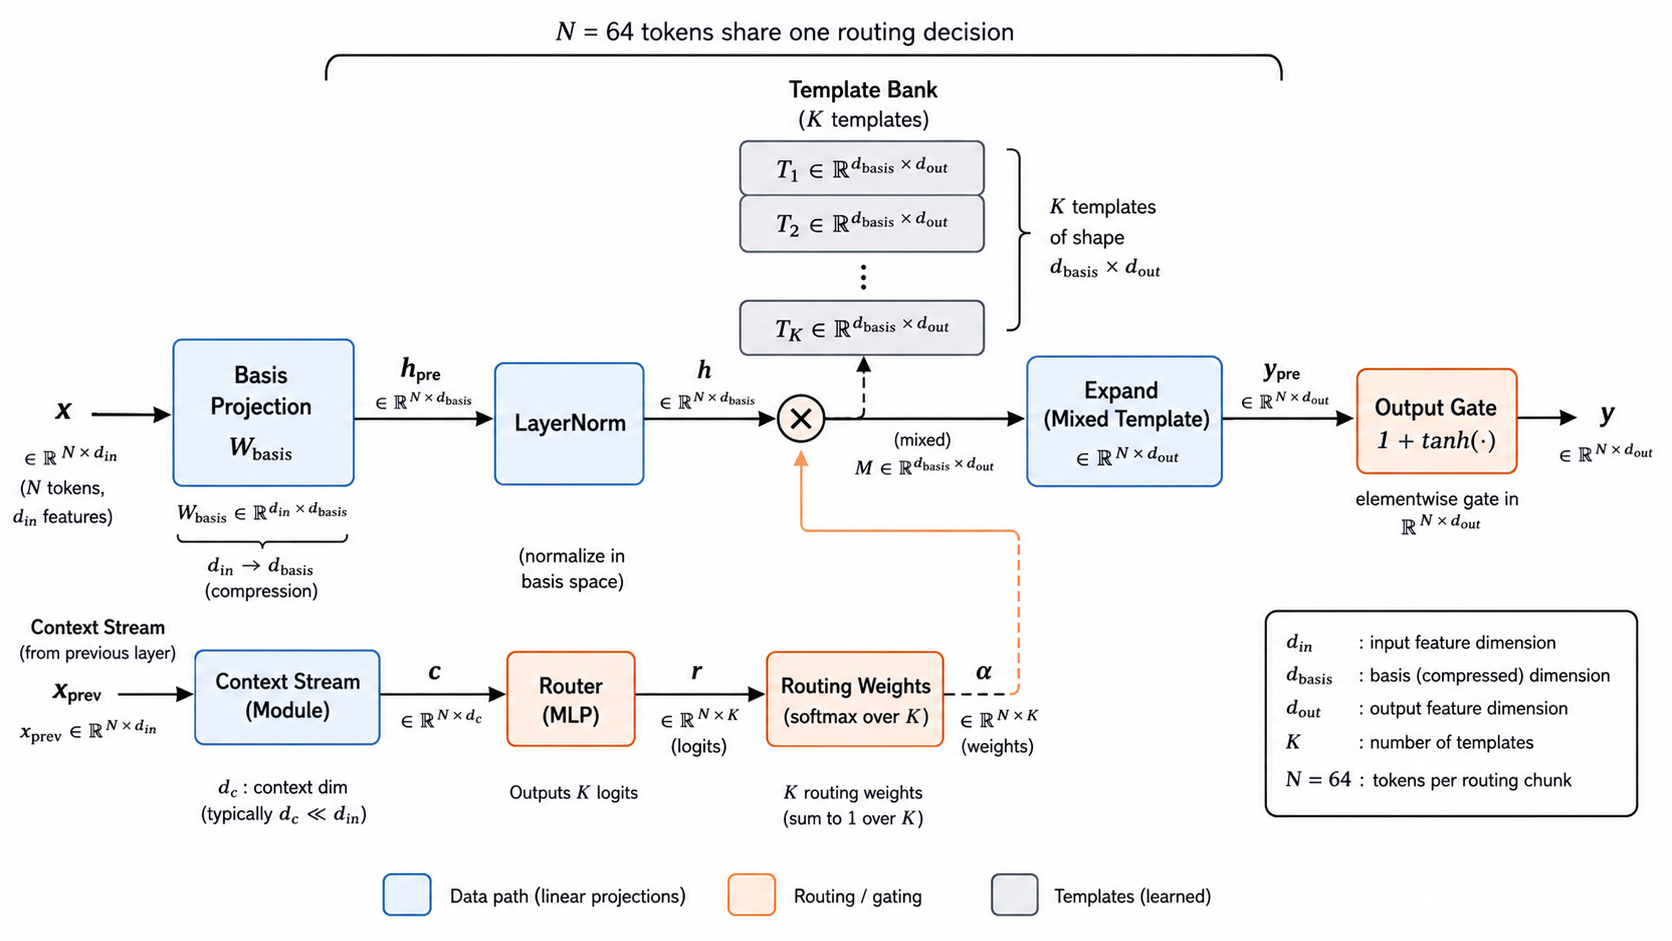
\includegraphics[width=0.95\textwidth]{remixedlinear_architecture.png}
    \caption{Architecture of the RemixedLinear layer. The data path (blue) compresses input $\mathbf{x}$ via a basis projection, normalizes it, then expands through a mixed template matrix. The context stream (orange) produces routing weights $\boldsymbol{\alpha}$ that select the template combination from a bank of $K$ learned templates (gray). Routing is amortized over chunks of $N{=}64$ tokens. A centered output gate ($1 + \tanh$) modulates the final output.}
    \label{fig:architecture}
\end{figure*}

\subsection{Overview}

A standard linear layer computes $\mathbf{y} = \mathbf{W}\mathbf{x} + \mathbf{b}$, where $\mathbf{W} \in \mathbb{R}^{d_\text{out} \times d_\text{in}}$ is a static matrix applied identically to all inputs. RemixedLinear replaces this with a dynamic composition:

\begin{equation}
\mathbf{y} = \left(\mathbf{W}_\text{eff}(\mathbf{c}) \cdot \text{LN}(\mathbf{W}_b \mathbf{x})\right) \odot \mathbf{g}_\text{out}(\mathbf{c}) + \mathbf{b}
\label{eq:remixedlinear}
\end{equation}

\noindent where $\mathbf{W}_b \in \mathbb{R}^{B \times d_\text{in}}$ is a basis projection ($B$ = basis size), $\mathbf{W}_\text{eff}(\mathbf{c})$ is a context-dependent effective mixing matrix constructed from $K$ templates, and $\mathbf{g}_\text{out}(\mathbf{c})$ is a low-rank output gate. The context signal $\mathbf{c}$ is derived from a causal context stream (Section~\ref{sec:context}).

\subsection{Template Mixing with Chunk Routing}
\label{sec:chunked}

RemixedLinear stores $K$ template matrices $\{\mathbf{T}_k\}_{k=1}^K$, each $\mathbf{T}_k \in \mathbb{R}^{d_\text{out} \times B}$. The effective mixing matrix is a weighted combination:

\begin{equation}
\mathbf{W}_\text{eff}(\mathbf{c}) = \sum_{k=1}^{K} \alpha_k(\mathbf{c}) \cdot \mathbf{T}_k
\end{equation}

\noindent where $\boldsymbol{\alpha}(\mathbf{c}) = \text{softmax}(\mathbf{W}_r \mathbf{c} / \tau)$ are routing weights computed from the context signal, $\mathbf{W}_r \in \mathbb{R}^{K \times d_\text{in}}$ is a learned routing projection, and $\tau$ is a temperature parameter.

\paragraph{Chunk amortization.} Per-token routing introduces two problems: high FLOPs overhead from computing $\boldsymbol{\alpha}$ for every token, and gradient instability from the multiplicative coupling between routing weights and template gradients. We amortize routing over chunks of $N{=}64$ tokens: the routing weights $\boldsymbol{\alpha}$ are computed once from the \emph{first token} of each chunk and shared across all tokens in that chunk. Because the anchor is the chunk's earliest token, no future information leaks into the routing decision, preserving the autoregressive causal constraint. This reduces routing FLOPs by a factor of $N$ and stabilizes training by decoupling routing updates from per-token gradient noise.

\paragraph{Quantile-balanced routing.}
Standard MoE requires auxiliary load-balancing losses to prevent expert collapse \citep{fedus2022switch}. We replace this with quantile-balanced routing. Concretely, we maintain a per-expert EMA threshold $\boldsymbol{\theta}_k$ updated each step as $\boldsymbol{\theta}_k \leftarrow \lambda\,\boldsymbol{\theta}_k + (1{-}\lambda)\,q_k$, where $q_k$ is the $(1 - \text{topk}/K)$-quantile of expert $k$'s batch scores and $\lambda{=}0.99$. A token is assigned to expert $k$ if its score exceeds $\boldsymbol{\theta}_k$, unioned with a hard top-$k$ fallback to guarantee at least $k$ active experts per token; excess selections are trimmed to the highest-scoring $k$.

We state the differentiability precisely, since it is easy to overclaim. Thresholding scores against $\boldsymbol{\theta}_k$ is a discrete operation and receives no gradient, exactly as in top-$k$ MoE; $\boldsymbol{\theta}_k$ is a non-learned running statistic, not a parameter. What is differentiable is the \emph{weighting over the selected templates}, through the masked softmax, so the router is trained by gradients flowing through the coefficients of templates that were selected, not through the selection itself. When all $K$ templates are selected (the configuration we ship, $\text{topk}{=}0$) the mask is vacuous and routing is fully differentiable softmax mixing.

We also flag a limitation of this criterion that we did not appreciate when designing it. Because the thresholded set is \emph{unioned} with the hard top-$k$ set, and the top-$k$ entries by construction hold the largest scores, the subsequent re-selection returns exactly those same entries whatever the threshold admitted: the balancing criterion cannot displace a top-$k$ template. In our implementation it is therefore numerically identical to plain top-$k$ routing with a softmax, and any balanced utilization we observe is a property of the learned router rather than of this mechanism. Section~\ref{sec:ablations} reports the corresponding ablation. Displacing rather than unioning is the natural fix and we leave it to future work.

\subsection{Centered Output Gate}
\label{sec:gate}

A low-rank output gate modulates the output:
\begin{equation}
\mathbf{g}_\text{out}(\mathbf{c}) = 1 + \tanh\!\left(s \cdot (\mathbf{W}_c \mathbf{c})^\top \mathbf{G}\right)
\end{equation}

\noindent where $\mathbf{W}_c \in \mathbb{R}^{r \times d_c}$ projects the context vector to $r$ coefficients, $\mathbf{G} \in \mathbb{R}^{r \times d_\text{out}}$ is a learned basis, $d_c$ is the context stream dimension, $r{=}8$ is the gate rank, and $s$ is a learned scalar initialized to 0.1. The $1 + \tanh(\cdot)$ formulation, with $\mathbf{W}_c$ and $\mathbf{G}$ zero-initialized, ensures $\mathbf{g}_\text{out} = \mathbf{1}$ at initialization. This is critical: it guarantees that RemixedLinear produces \emph{output-equivalent} results to a standard linear layer at step~0 (up to the intermediate LayerNorm; see Section~\ref{sec:ln_confound}), avoiding the optimization friction that caused all sigmoid-gated designs to fail in our ablation studies (Appendix~\ref{app:evolution}).

\subsection{Context Stream}
\label{sec:context}

The context signal $\mathbf{c}$ is derived from a causal context stream that maintains a running representation across the sequence. We use a \emph{selective} stream with GRU-style gating:
\begin{equation}
\mathbf{c}_t = (1 - \mathbf{z}_t) \odot \mathbf{c}_{t-1} + \mathbf{z}_t \odot \tilde{\mathbf{c}}_t
\end{equation}

\noindent where $\mathbf{z}_t = \sigma(\mathbf{W}_z \mathbf{x}_t)$ is an input-dependent update gate ($\mathbf{W}_z \in \mathbb{R}^{d_c \times d}$) and $\tilde{\mathbf{c}}_t = \tanh(\mathbf{W}_w \mathbf{x}_t)$ is the candidate state ($\mathbf{W}_w \in \mathbb{R}^{d_c \times d}$, zero-initialized so that $\tilde{\mathbf{c}}_0 = \mathbf{0}$ at initialization). The context state is \emph{detached} between steps to prevent gradient explosion through long recurrent chains, a lesson from Phase~3 of our ablation study (Appendix~\ref{app:evolution}).

\subsection{Integration into the Transformer Block}

RemixedLinear replaces all six linear projections in each Transformer block: Q, K, V, attention output projection, and both FFN layers ($\mathbf{W}_\text{fc}$, $\mathbf{W}_\text{proj}$). Each projection has its own set of $K$ templates and routing weights, allowing different projections to specialize independently. The context stream is shared within each block.

\subsection{Complexity Analysis}

Table~\ref{tab:flops} compares per-token FLOPs for a single projection.

\begin{table}[t]
\centering
\small
\caption{FLOPs per token for a single linear projection with $d_\text{in} = d_\text{out} = d$, basis size $B = d$, $K$ templates, chunk size $N$, context dimension $d_c$, gate rank $r$.}
\label{tab:flops}
\begin{tabular}{@{}lc@{}}
\toprule
\textbf{Component} & \textbf{FLOPs} \\
\midrule
Dense baseline ($\mathbf{W}\mathbf{x}$) & $2d^2$ \\
\midrule
Basis projection ($\mathbf{W}_b \mathbf{x}$) & $2dB$ \\
Template assembly ($\sum \alpha_k \mathbf{T}_k$, amort.) & $2KBd/N$ \\
Template mixing ($\mathbf{W}_\text{eff} \mathbf{h}$) & $2Bd$ \\
Routing (amortized, $1/N$) & $2d_c K/N$ \\
Output gate (rank $r$) & $2(d_c r + rd)$ \\
\midrule
\textbf{Total (RemixedLinear)} & $\approx 4dB + 2r(d_c{+}d)$ \\
\bottomrule
\end{tabular}
\end{table}

With $B = d$ (full-rank basis, as used in all experiments), RemixedLinear uses approximately $4d^2$ active FLOPs per projection versus $2d^2$ for dense, a $2\times$ per-projection overhead. However, the model stores $K$ template matrices totaling $K \cdot B \cdot d$ parameters while the active computation per token uses only the weighted sum of templates plus the basis projection. The ratio of stored parameters to per-token active parameters is $(K \cdot B \cdot d + B \cdot d) / (B \cdot d + B \cdot d) = (K{+}1)/2$ for full-rank $B{=}d$, enabling the model to express a richer family of transformations from a larger parameter bank while maintaining bounded inference cost.

\section{Experiments}
\label{sec:experiments}

\subsection{Setup}

\paragraph{Framework.} All experiments use nanochat \citep{karpathy2025nanochat}, a single-file GPT implementation supporting Flash Attention \citep{dao2022flashattention}, bf16 mixed precision, and the Muon optimizer \citep{jordan2024muon} for matrix-shaped parameters with AdamW for embeddings and scalars.

\paragraph{Dataset.} ClimbMix \citep{nvidia2024climbmix}, a curated pretraining mixture, tokenized with a 32,768-vocabulary BPE tokenizer. Sequence length is 2048 tokens.

\paragraph{Training horizon.} Following Chinchilla scaling \citep{hoffmann2022training}, each model is trained with a fixed 10.5$\times$ token-to-scaling-parameter ratio, where scaling parameters exclude embedding tables. This ensures compute-optimal training at every scale.

\paragraph{Metric.} Validation bits-per-byte (BPP), a vocabulary-size-invariant measure of language model quality. Lower is better.

\paragraph{Model scales.} We evaluate at three scales. In nanochat, the ``depth'' parameter serves dual duty: it sets both the number of Transformer layers ($n_\text{layer} = \text{depth}$) and the base model width ($d = \text{depth} \times 64$, rounded up to the nearest multiple of the head dimension 128). All experiments use full-rank basis $B = d$, context dimension $d_c = d$, output gate rank $r = 8$ (matching Section~\ref{sec:gate}), and head dimension 128.

\begin{table}[t]
\centering
\small
\caption{Model configurations. RemixedLinear uses $K{=}8$ templates, chunk size $N{=}64$, quantile routing ($\lambda{=}0.99$), selective context stream, and full-rank basis $B{=}d$.}
\label{tab:configs}
\begin{tabular}{@{}lccc@{}}
\toprule
& \textbf{d4} & \textbf{d8} & \textbf{d12} \\
\midrule
Layers ($n_\text{layer}$) & 4 & 8 & 12 \\
Model dim ($d$) & 256 & 512 & 768 \\
Basis size ($B$) & 256 & 512 & 768 \\
Heads & 2 & 4 & 6 \\
Dense params & $\sim$37M & $\sim$126M & $\sim$286M \\
Remix total params & 56M & 276M & 792M \\
Remix active params & 37M & 127M & 290M \\
Training tokens & $\sim$0.4B & $\sim$1.3B & $\sim$3.0B \\
\bottomrule
\end{tabular}
\end{table}

\paragraph{Baselines.} (1) Dense Transformer baseline (nanochat default) at depths 12 through 30. (2) Standard MoE with 8 experts, top-1 and top-all routing at depth 4.

\subsection{Main Results}

Table~\ref{tab:main} presents the primary comparison.

\begin{table}[t]
\centering
\small
\caption{Main results. RemixedLinear consistently outperforms the dense baseline at matched active FLOPs across all three scales. Standard MoE underperforms the dense baseline at d4.}
\label{tab:main}
\begin{tabular}{@{}lcccc@{}}
\toprule
\textbf{Model} & \textbf{Total} & \textbf{Active} & \textbf{FLOPs} & \textbf{BPP} \\
& \textbf{Params} & \textbf{Params} & & \\
\midrule
\multicolumn{5}{l}{\textit{Dense baselines}} \\
\quad Dense d4 & 37M & 37M & 7.8e7 & 1.170 \\
\quad Dense d8 & 126M & 126M & 2.9e8 & 0.969 \\
\quad Dense d12 & 286M & 286M & 7.6e8 & 0.903 \\
\midrule
\multicolumn{5}{l}{\textit{RemixedLinear (ours)}} \\
\quad Remix d4 & 56M & 37M & 9.4e7 & \textbf{1.082} \\
\quad Remix d8 & 276M & 127M & 4.1e8 & \textbf{0.903} \\
\quad Remix d12 & 792M & 290M & 1.1e9 & \textbf{0.814} \\
\midrule
\multicolumn{5}{l}{\textit{Standard MoE (d4 only)}} \\
\quad MoE top-1 & 51M & 37M & 7.8e7 & 1.187 \\
\quad MoE top-all & 51M & 51M & 1.7e8 & 1.186 \\
\bottomrule
\end{tabular}
\end{table}

At every scale, RemixedLinear achieves lower BPP than the dense baseline at comparable active FLOPs. The improvement is consistent across scales but we see no evidence that it grows: the relative gaps are 7.5\% at d4, 6.8\% at d8 and 9.9\% at d12, and in absolute BPP they are 0.088, 0.066 and 0.089, which is flat and non-monotonic. With one seed per configuration we cannot distinguish this variation from run-to-run noise, and we make no claim about a scaling trend in the gap. Notably, RemixedLinear at d8 (0.903 BPP, 127M active params) matches the dense d12 baseline (0.903 BPP, 286M params), achieving equivalent quality with 2.25$\times$ fewer active parameters.

Standard MoE at d4 performs \emph{worse} than the dense baseline (1.187 vs. 1.170 BPP), despite having 51M total parameters. This suggests that coarse-grained expert routing at the FFN level is insufficient at this scale, while RemixedLinear's fine-grained template routing within individual projections provides a qualitatively different advantage.

\subsection{Scaling Law Analysis}

\begin{figure*}[t]
    \centering
    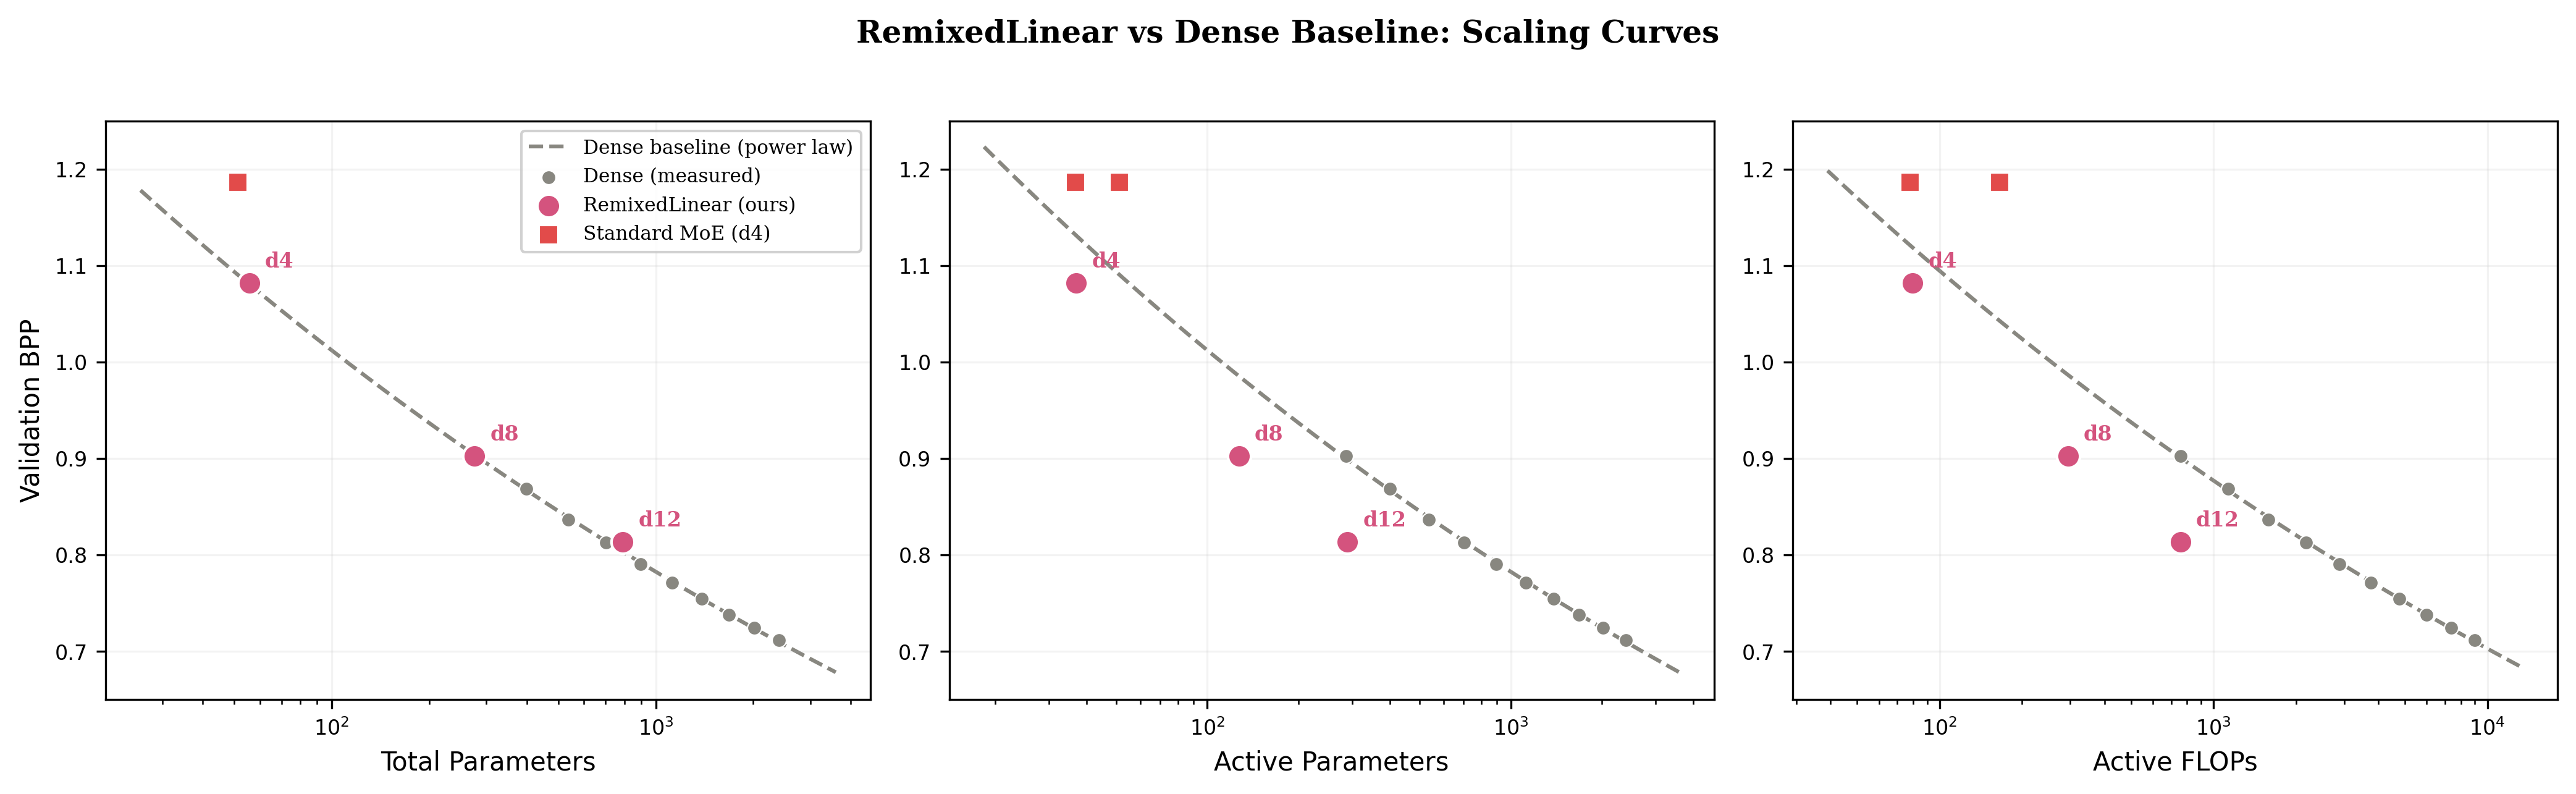
\includegraphics[width=0.95\textwidth]{scaling_curves_acl.png}
    \caption{Validation BPP vs.\ total parameters (left), active parameters (center), and active FLOPs (right). Dashed lines show power-law fits to dense baselines (d12--d30). RemixedLinear points (pink circles) fall consistently below the dense scaling curve, indicating better compute efficiency. Standard MoE (red squares) falls above the curve at d4.}
    \label{fig:scaling}
\end{figure*}

Figure~\ref{fig:scaling} plots BPP against total parameters, active parameters, and active FLOPs. The dense baseline (d12--d30) follows a tight power law $\text{BPP} = a \cdot \text{FLOPs}^b$. RemixedLinear points fall consistently below this curve when measured against active FLOPs, confirming that the architecture achieves genuine compute efficiency gains rather than merely trading parameters for quality.

The d12 RemixedLinear point is particularly striking: at nearly identical active FLOPs to the dense d12 baseline ($7.58 \times 10^8$ vs.\ $7.60 \times 10^8$), it achieves 0.814 BPP versus 0.903, matching the dense power-law extrapolation at approximately d20 scale ($\sim$900M params, $\sim 2.9 \times 10^9$ FLOPs).

\subsection{Ablation Study}
\label{sec:ablations}

To isolate the contribution of each design component, we run ablations at d4 using the P29 sweep configuration. Table~\ref{tab:ablation} reports results for the key variants tested.

\begin{table}[t]
\centering
\small
\caption{Ablation study at d4. \emph{Top}: routing variants with $K{=}8$ templates. \emph{Middle}: gate component ablation with $K{=}1$ template (isolating gate effects from routing). \emph{Bottom}: standard MoE baselines. $\Delta$ is relative to the dense baseline BPP of 1.170.}
\label{tab:ablation}
\begin{tabular}{@{}lcc@{}}
\toprule
\textbf{Configuration} & \textbf{BPP} & \textbf{$\Delta$} \\
\midrule
Dense baseline & 1.170 & -- \\
\midrule
\multicolumn{3}{l}{\textit{Routing variants ($K{=}8$ templates)}} \\
\quad 29A: Top-1 routing (per-token) & 1.087 & $-$7.1\% \\
\quad 29C: Chunk-64 routing & \textbf{1.082} & $-$7.5\% \\
\quad 29E: Top-1 + Chunk-64 & 1.082 & $-$7.5\% \\
\quad 29H: 4 templates, dense mix & 1.127 & $-$3.7\% \\
\midrule
\multicolumn{3}{l}{\textit{Gate component ablation ($K{=}1$)}} \\
\quad No context, no gates & 1.168 & $-$0.2\% \\
\quad Output gate + context only & 1.165 & $-$0.4\% \\
\quad + Linear basis gate & 1.160 & $-$0.9\% \\
\midrule
\multicolumn{3}{l}{\textit{Standard MoE ($K{=}8$ experts)}} \\
\quad MoE top-1 & 1.187 & $+$1.5\% \\
\quad MoE top-all & 1.186 & $+$1.4\% \\
\bottomrule
\end{tabular}
\end{table}

\paragraph{Chunk routing matches per-token.} Configurations 29A (per-token top-1) and 29C (chunk-64) achieve nearly identical BPP (1.087 vs. 1.082), while chunk routing uses substantially fewer routing FLOPs. The combined variant (29E) shows no additional benefit, confirming that chunk-64 captures the useful routing structure.

\paragraph{Template count matters.} Reducing from $K{=}8$ to $K{=}4$ templates (29H) degrades BPP from 1.082 to 1.127, though it still outperforms the dense baseline. This suggests the model benefits from a diverse set of template specializations.

\paragraph{Gate contributions are modest but additive.} With a single template ($K{=}1$), the basis-mixing factorization alone already matches the dense baseline (1.168 vs. 1.170). Note that the $K{=}1$ variant includes an intermediate LayerNorm between the basis projection and the mixing matrix (Eq.~\ref{eq:remixedlinear}), which is absent from the dense baseline; we investigate this confound in Section~\ref{sec:ln_confound}. Adding the output gate and context stream improves BPP to 1.165, and further adding a linear basis gate reaches 1.160. The basis gate thus contributes only 0.005 BPP improvement at significant FLOPs cost ($\sim$0.625$d^2$ per projection); we omit it in the final architecture, relying on the output gate and context stream for modulation while template routing provides the primary performance gain.

\paragraph{Standard MoE fails at this scale.} Both MoE variants underperform the dense baseline, consistent with the established empirical finding that MoE requires ${\geq}$1B active parameters before outperforming dense models \citep{fedus2022switch}. Expert specialization does not emerge at small scale, and the routing overhead and auxiliary loss introduce additional friction that a dense model avoids.

\subsection{Inference Throughput}
\label{sec:throughput}

While RemixedLinear improves quality at matched \emph{active} FLOPs, its wall-clock inference throughput is lower than the dense baseline. Table~\ref{tab:throughput} reports measurements on a single NVIDIA H200 GPU at batch size 64, sequence length 2048, without \texttt{torch.compile}.

\begin{table}[t]
\centering
\small
\caption{Inference throughput at d12 on a single H200 GPU (batch 64, seq 2048). Hardware FLOPs are measured via \texttt{torch.utils.flop\_counter}. RemixedLinear achieves 10\% better BPP but at 3.7$\times$ lower throughput. GPU utilization (measured TFLOPS) drops from 195 to 86, suggesting the GPU's compute units are substantially underutilized in the RemixedLinear forward pass.}
\label{tab:throughput}
\begin{tabular}{@{}lcc@{}}
\toprule
\textbf{Metric} & \textbf{Dense d12} & \textbf{Remix d12} \\
\midrule
Total params & 286M & 792M \\
Active params & 286M & 290M \\
HW FLOPs/token & $2.2 \times 10^8$ & $3.6 \times 10^8$ \\
Throughput (tok/s) & 886k & 242k \\
Peak memory (GB) & 49.3 & 53.5 \\
GPU utilization (TFLOPS) & 195 & 86 \\
Val BPP & 0.903 & 0.814 \\
\bottomrule
\end{tabular}
\end{table}

The hardware FLOP ratio is only 1.6$\times$ (3.6e8 vs.\ 2.2e8), yet throughput differs by 3.7$\times$. The GPU utilization drops from 195 to 86 TFLOPS, indicating that RemixedLinear's compute units are substantially idle during inference. Module-level profiling reveals that the slowdown is distributed across all RemixedLinear projections: attention (Q/K/V/O) is ${\sim}$5$\times$ slower per layer and FFN is ${\sim}$8$\times$ slower, consistent with each RemixedLinear replacing a single cuBLAS GEMM with multiple operations (template stacking, routing, weight composition via einsum, and a second einsum for the output). We attempted fused Triton kernels to eliminate the intermediate $W_\text{eff}$ materialization, but the custom kernel was 3$\times$ slower than the cuBLAS-backed PyTorch baseline, as the hand-tuned tiling cannot match cuBLAS's optimized memory coalescing and warp scheduling for these matrix shapes.

Closing this throughput gap is the primary practical challenge for deployment, and we report a negative result on the most obvious route. We implemented the batched-GEMM reformulation: with top-1 routing there are at most $K$ distinct effective weights per forward, so chunks can be permuted into template-contiguous order and dispatched as $K$ dense GEMMs against the bank (\texttt{torch.\_grouped\_mm}), never materializing a per-chunk weight matrix. The implementation is bit-exact against the composed path and compiles without graph breaks. It does not improve end-to-end training throughput at d4 or d12: the permutation gather in the forward pass and its scatter in the backward pass together cost about as much as the eliminated weight traffic at the basis-to-chunk ratios we train at. We note this because the slowdown is often assumed to be an implementation artifact; on the evidence we have it is closer to intrinsic. We previously suggested distilling to $K{=}1$ at inference time. As literally stated that is incoherent, since $K{=}1$ \emph{is} a dense layer and scores 1.168 BPP at d4 against the dense baseline's 1.170. The coherent version is distilling a $K{=}8$ teacher into a dense student, which is a different and untested claim; we flag it as future work rather than a fix in hand.

\subsection{Downstream Task Evaluation}
\label{sec:core}

To verify that BPP improvements translate to genuine downstream task performance, we evaluate all models on the CORE benchmark \citep{li2024dclm}, a standardized suite of 22 in-context learning tasks from the DataComp for Language Models (DCLM) framework. The CORE metric uses \emph{centered accuracy}: each task's raw accuracy is linearly rescaled so that random guessing maps to 0 and perfect accuracy to 1, enabling meaningful averaging across tasks with different baselines.

The 22 tasks span commonsense reasoning (HellaSwag, PIQA, WinoGrande, Winograd, COPA, CommonsenseQA, OpenBookQA), world knowledge (ARC-Easy, ARC-Challenge, Jeopardy, BigBench QA WikiData), reading comprehension (BoolQ, SQuAD, CoQA, LAMBADA), algorithmic reasoning (BigBench Dyck Languages, CS Algorithms, Operators, Repeat Copy Logic), and logical/linguistic reasoning (AGI Eval LSAT-AR, BigBench Language Identification). Table~\ref{tab:core} reports aggregate CORE scores.

\begin{table}[t]
\centering
\small
\caption{CORE benchmark scores (22-task centered accuracy aggregate). Higher is better. Dense d14--d30 are nanochat leaderboard runs. The dense d12 entry here differs from our own d12 dense checkpoint, which scores 0.146; see the ``Which dense baseline'' paragraph and Table~\ref{tab:core_pertask}, and prefer the measured comparison given there.}
\label{tab:core}
\begin{tabular}{@{}lcccc@{}}
\toprule
\textbf{Model} & \textbf{Active Params} & \textbf{Active FLOPs} & \textbf{Val BPP} & \textbf{CORE} \\
\midrule
Dense d12 & 286M & 7.6e8 & 0.903 & 0.114 \\
Dense d14 & 399M & 1.1e9 & 0.869 & 0.148 \\
Dense d20 & 897M & 2.9e9 & 0.791 & 0.215 \\
Dense d26 & 1.68B & 6.0e9 & 0.738 & 0.266 \\
Dense d30 & 2.40B & 9.0e9 & 0.712 & 0.291 \\
\midrule
Remix d8 & 127M & 4.1e8 & 0.903 & \textbf{0.123} \\
Remix d12 & 290M & 1.1e9 & 0.814 & \textbf{0.172} \\
\bottomrule
\end{tabular}
\end{table}

\begin{figure*}[t]
    \centering
    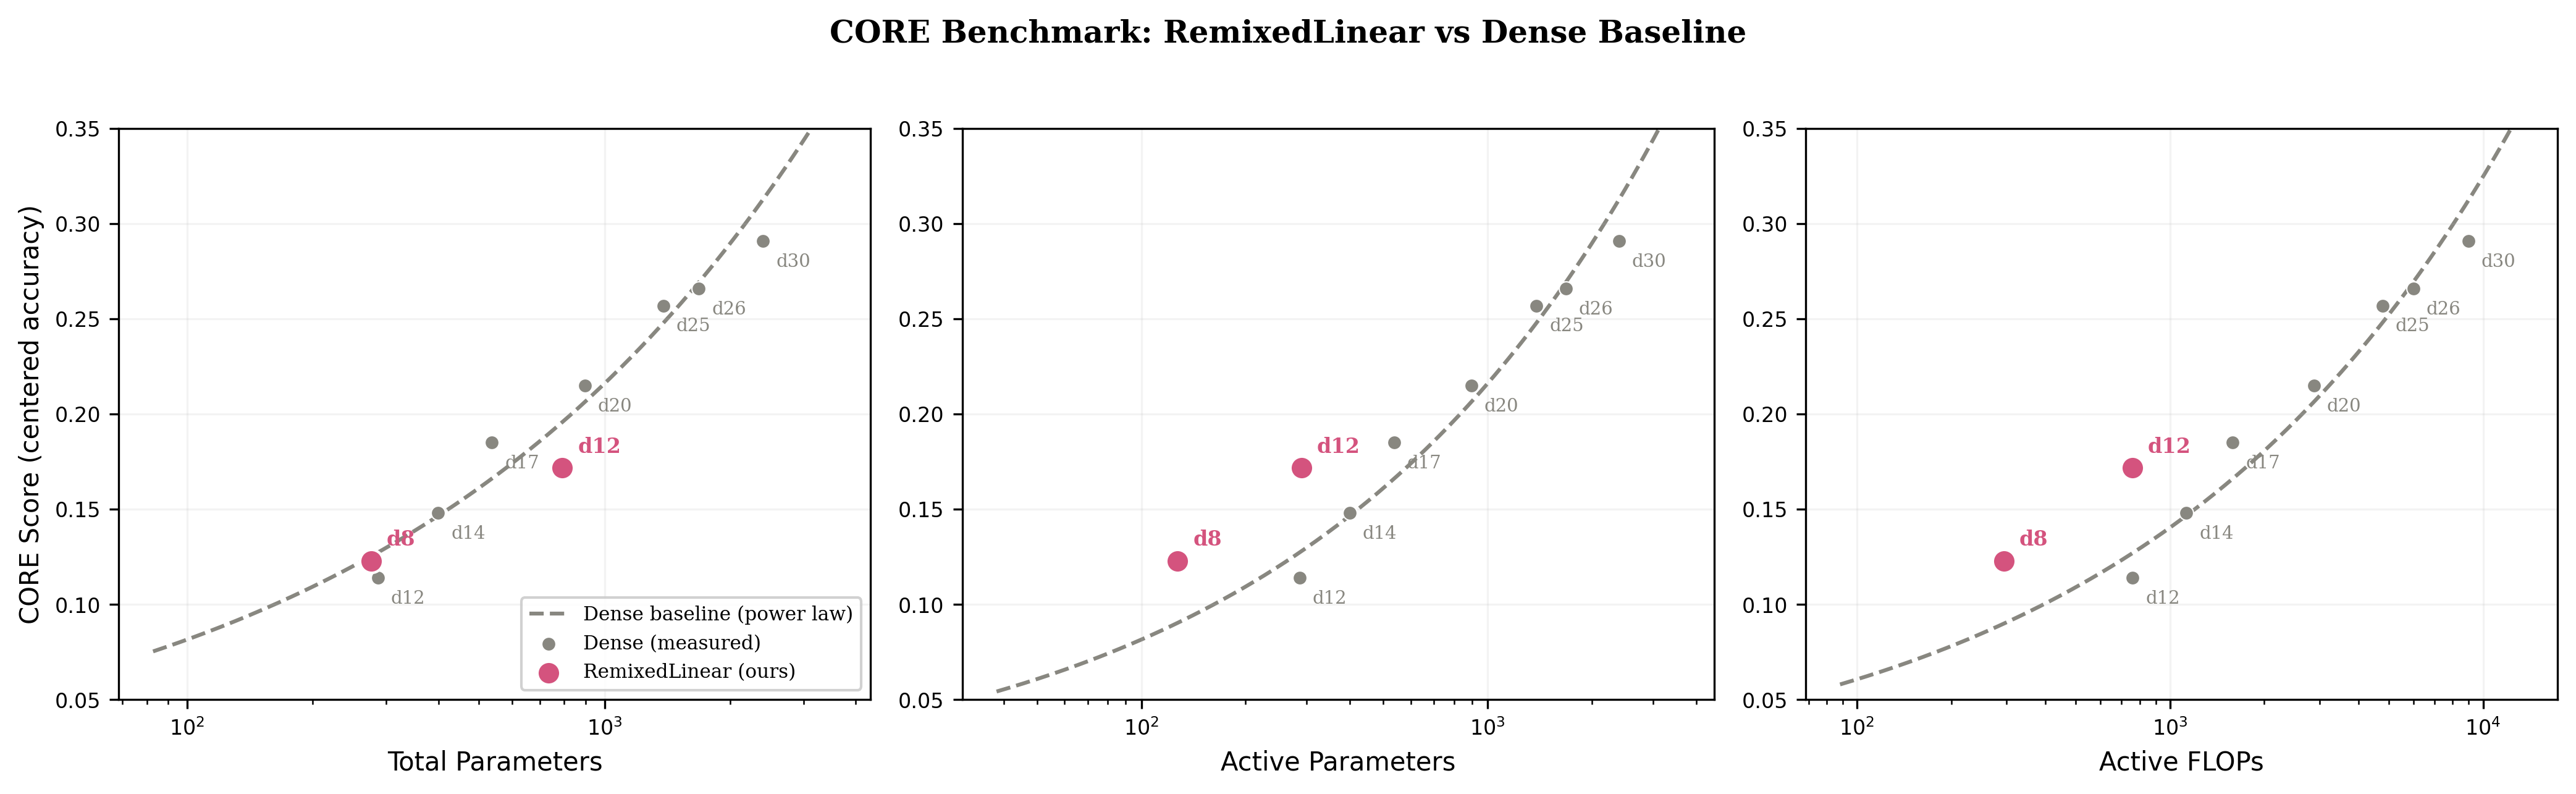
\includegraphics[width=0.95\textwidth]{scaling_curves_core.png}
    \caption{CORE score vs.\ model size and compute. \textbf{Left:} Total parameters --- Remix falls on the dense curve, reflecting $K{\times}$ storage. \textbf{Middle/Right:} Active parameters and active FLOPs --- Remix sits above the dense power-law fit at matched compute, indicating the improvement is not a parameter-counting artifact. Note the fit under-predicts the measured dense d12--d14 points; against measured baselines the gain is $+0.025$ centered accuracy (Section~\ref{sec:core}).}
    \label{fig:core_scaling}
\end{figure*}

Figure~\ref{fig:core_scaling} plots CORE score against active FLOPs. Relative to the dense power-law fit, Remix d8 sits 36\% above the prediction (0.123 vs.\ 0.090) and Remix d12 35\% above (0.172 vs.\ 0.127). We report these for continuity with the scaling analysis but do not lead with them: as the following paragraphs set out, the fit under-predicts the measured dense points near d12--d14, and against measured baselines the gain is $+0.025$ centered accuracy. The directionally useful statement is that BPP improvements do transfer to downstream tasks, on 17 of 22 tasks individually.

\paragraph{Per-task breakdown.} R5 asked whether the aggregate CORE gain is broad or concentrated in a few tasks. Table~\ref{tab:core_pertask} reports all 22 tasks. Remix d12 exceeds our dense d12 baseline on 17, trails on 4 and ties on 1, so the gain is broad rather than driven by a handful of tasks. It is not uniform: BoolQ regresses sharply ($-0.284$ centered), and it is the only task on which either model sits well below chance, which is worth noting because BoolQ's centered scale amplifies sub-random accuracy. We also report absolute differences alongside relative ones, since at this scale most CORE tasks sit near random and a percentage on a near-zero base overstates the effect: the d12 aggregate difference is $+0.026$ absolute.

\paragraph{Which dense baseline.} We flag an inconsistency in our own numbers rather than leave it for the reader to find. The dense d12 CORE score in Table~\ref{tab:core} is 0.114, while the per-task evaluation in Table~\ref{tab:core_pertask}, run on our own dense d12 checkpoint, aggregates to 0.146. The two were produced from different checkpoints and we regard the 0.146 figure, for which we can report every task, as the one to compare against. On that basis the d12 CORE gain is $+0.026$ absolute rather than $+0.058$, and the ``34--36\% above the dense power-law prediction'' framing should be read against the power-law fit rather than against a measured dense model.

\begin{table}[t]
\centering
\small
\caption{Per-task CORE centered accuracy. Requested by R5. Remix d12 exceeds our dense d12 baseline on 17 of 22 tasks and trails on 4. The aggregate gain is broad rather than concentrated in a few tasks, but it is not uniform: BoolQ is a large regression, and it is the only task where either model is far below random. Centered accuracy rescales each task so random guessing is 0; negative values are below chance.}
\label{tab:core_pertask}
\begin{tabular}{lrrrr}
\toprule
\textbf{Task} & \textbf{Dense d12} & \textbf{Remix d8} & \textbf{Remix d12} & \textbf{$\Delta$ d12} \\
\midrule
HellaSwag (0-shot) & 0.136 & 0.112 & \textbf{0.205} & +0.069 \\
Jeopardy & 0.008 & 0.002 & \textbf{0.022} & +0.014 \\
BigBench QA WikiData & 0.294 & 0.216 & \textbf{0.370} & +0.076 \\
ARC-Easy & 0.392 & 0.360 & \textbf{0.491} & +0.099 \\
ARC-Challenge & 0.035 & 0.027 & \textbf{0.077} & +0.043 \\
COPA & 0.180 & 0.020 & \textbf{0.260} & +0.080 \\
CommonsenseQA & 0.065 & 0.185 & \textbf{0.240} & +0.175 \\
PIQA & 0.352 & 0.316 & \textbf{0.380} & +0.028 \\
OpenBookQA & 0.072 & 0.051 & \textbf{0.120} & +0.048 \\
LAMBADA & 0.282 & 0.268 & \textbf{0.344} & +0.062 \\
HellaSwag & 0.136 & 0.104 & \textbf{0.213} & +0.077 \\
Winograd & 0.187 & 0.114 & 0.143 & -0.044 \\
WinoGrande & 0.024 & 0.008 & \textbf{0.028} & +0.004 \\
BigBench Dyck Languages & 0.068 & 0.018 & \textbf{0.070} & +0.002 \\
AGI Eval LSAT-AR & 0.005 & 0.038 & \textbf{0.082} & +0.076 \\
BigBench CS Algorithms & 0.442 & 0.452 & 0.426 & -0.016 \\
BigBench Operators & 0.095 & 0.100 & \textbf{0.114} & +0.019 \\
BigBench Repeat Copy Logic & 0.031 & 0.000 & 0.031 & +0.000 \\
SQuAD & 0.206 & 0.140 & \textbf{0.218} & +0.012 \\
CoQA & 0.158 & 0.158 & \textbf{0.196} & +0.038 \\
BoolQ & -0.147 & -0.184 & -0.432 & -0.284 \\
BigBench Language ID & 0.184 & 0.199 & 0.179 & -0.004 \\
\midrule
\textbf{CORE (aggregate)} & 0.146 & 0.123 & \textbf{0.172} & +0.026 \\
\bottomrule
\end{tabular}
\end{table}


\section{Discussion}

\paragraph{Why fine-grained routing outperforms coarse MoE.}
RemixedLinear operates within each linear projection (six per block), providing $6{\times}K$ effective routing decisions per block rather than one per FFN. We note that the advantage is primarily from this granularity and chunk amortization rather than from continuous vs.\ discrete routing: ablation 29E shows top-1 chunk routing matches soft routing at 1.082 BPP. Both substantially outperform coarse FFN-level MoE at the scales tested.

\paragraph{The optimization friction problem.}
Our 29-phase ablation history (Appendix~\ref{app:evolution}) documents a systematic pattern: multiplicative sigmoid gating that modulated individual basis features through learned per-token routing consistently degraded training (Phases 4--9). The final design resolves this by routing over $K$ template-level softmax weights rather than per-feature sigmoid gates. Per-token learned routing (29A) works well in this formulation (1.087 BPP), and chunk-amortized routing (29C) achieves equivalent quality (1.082) at lower cost.

\paragraph{LayerNorm confound.}
\label{sec:ln_confound}
RemixedLinear applies an intermediate LayerNorm between the basis projection and the mixing matrix, absent from the dense baseline. At $K{=}1$ with no context or gates, the 0.002 BPP improvement (1.168 vs.\ 1.170) may partly reflect this normalization benefit rather than the factored structure. A controlled ablation adding an intermediate LayerNorm to the dense baseline would isolate this effect; we leave it to future work.

\paragraph{Limitations.}
Our RemixedLinear scaling curve spans only three points (d4, d8, d12); confirming gains at d20+ ($\sim$1B active parameters) remains essential future work. The MoE comparison is limited to d4 due to compute constraints. All experiments were conducted without institutional compute resources across heterogeneous GPU hardware (A100, H100, H200, T4); dense baseline scores are from the published nanochat leaderboard \citep{karpathy2025nanochat}. The total parameter count of RemixedLinear models is $K{\times}$ larger than dense equivalents; while active parameters and FLOPs are matched, memory footprint and inference latency are higher (Section~\ref{sec:throughput}).

\section{Conclusion}

We introduced RemixedLinear, a drop-in replacement for dense linear layers that dynamically composes $K$ template matrices per chunk of tokens using content-aware routing. Through 29 phases of ablation, chunk-amortized routing, quantile balancing, and centered output gating emerged as the critical design choices. At d12 scale, RemixedLinear achieves 10\% lower BPP and 35\% higher CORE score than the dense baseline at matched active FLOPs, while standard MoE underperforms the baseline. Inference throughput is 3.7$\times$ lower than dense, and the batched-GEMM reformulation we implemented does not recover it; on current evidence the throughput cost should be treated as part of the method rather than as an implementation artifact. Scoped honestly, the claim we can defend is a quality gain at matched \emph{active parameters} and at matched \emph{measured} FLOPs, not at matched wall-clock.

\begin{ack}
In accordance with the AI Writing Assistance Policy, we acknowledge the use of large language models to assist with text editing. All content was reviewed and verified by the human author.
\end{ack}

\bibliographystyle{plainnat}
\bibliography{references}

\clearpage
\appendix
\section{Design Evolution: From CCL to RemixedLinear}
\label{app:evolution}

The final RemixedLinear architecture emerged from 29 phases of systematic ablation, each testing a specific hypothesis about how to make context-conditioned linear layers work. This appendix summarizes the key phases and the lessons they produced.

\paragraph{Phase 1--2: Global Context Manager.}
The original design used a cross-attention mechanism to compute a global context vector for modulating all linear layers. This architecture showed strong early results but was later discovered to contain a \textbf{causal leakage bug}: the cross-attention looked into future tokens. Once the leak was fixed, the architecture failed to beat the dense baseline.

\paragraph{Phase 3: BPTT through context.}
Allowing gradient flow through the recurrent context stream (removing \texttt{.detach()}) caused gradient explosion. This established that \textbf{context states must be detached} between time steps.

\paragraph{Phase 4--8: Activation vs. weight modulation.}
DiT-style activation modulation (AdaRMSNorm), multi-scale temporal bottlenecks, cross-layer stale context, and boundary-gated updates were all tested. None matched the dense baseline. The core finding: \textbf{weight-level modulation is more expressive than activation-level modulation}, but the gating mechanism must not interfere with the primary gradient path.

\paragraph{Phase 9: The identity trap.}
When context is derived from the same $\text{norm}(\mathbf{x})$ that the FFN processes, multiplicative sigmoid gating collapses to identity. Additive residual designs (RAL) also failed despite identity-safe initialization, establishing that \textbf{zero-init does not guarantee zero friction} during training.

\paragraph{Phase 12--17: CKR and position routing.}
Causal Kernel Reparameterization (CKR) using position-only routing was the first design to beat the dense baseline (+0.02 BPP). However, this improvement could not be reproduced reliably and did not scale beyond $K{=}4$ branches. The lesson: \textbf{position conditioning has a low ceiling}, as RoPE already provides adequate positional information.

\paragraph{Phase 20--21: Frozen content routing.}
Low-Rank Composition with Frozen Basis (LRCFB) used a frozen random projection for content-dependent routing, achieving $-0.025$ BPP improvement. This validated that \textbf{content routing works if the routing projection does not receive gradients from the main loss}.

\paragraph{Phase 22--29: Template mixing and chunk routing.}
Building on LRCFB, we introduced learned templates with chunk routing, quantile balancing, and the centered output gate. The $1 + \tanh$ gate formulation was the final key ingredient, resolving the optimization friction that had blocked all prior sigmoid-gated designs. The canonical configuration ($K{=}8$, chunk-64, quantile routing) is the subject of this paper.

\paragraph{Summary of failure modes.}
\begin{itemize}
\item \textbf{FM1 (Gradient fracturing):} In early sigmoid-gated designs, learned per-feature routing coupled with feature weight gradients degraded training. The template softmax formulation avoids this by routing at the template level rather than the feature level.
\item \textbf{FM2 (Identity trap):} Context derived from $\text{norm}(\mathbf{x})$ collapses gating to identity.
\item \textbf{FM3 (Rank bottleneck):} Subspace restrictions (low-rank deltas, channel splitting) underperform full-rank alternatives.
\item \textbf{FM4 (Capacity tax):} At small scale, any parameter overhead for routing mechanics is proportionally too expensive.
\item \textbf{FM5 (Zero-init illusion):} Starting as identity does not prevent the added pathway from disrupting training once gradients flow.
\end{itemize}

The resolution to all five failure modes was the combination of (1) template-level softmax routing (replacing per-feature sigmoid gating) to resolve FM1, with optional chunk amortization for efficiency, (2) a detached causal context stream to avoid FM2, (3) full-rank templates to avoid FM3, (4) the centered output gate to avoid FM4 and FM5.

%%%%%%%%%%%%%%%%%%%%%%%%%%%%%%%%%%%%%%%%%%%%%%%%%%%%%%%%%%%%
\newpage
\input{checklist.tex}

\end{document}
